\documentclass[openany]{book}
\input{notes_white}
\usepackage{mathtools}
\usepackage{pgfplots}
\usepackage{chemfig}
\settitle{Biology Lab Manual - Expt 4}
\begin{document}
\title{\Large{\underemphasise{Biology - Expt 4}} \\ \vspace{5pt}
\large{Estimation of Glucose Concentration using GOD-POD Assay}}
\author{Eklavya Raman \\ \vspace{5pt} er24ms024@iiserkol.ac.in \\ \vspace{5pt} \and Shrey Patnaik \\ \vspace{5pt} sp24ms174@iiserkol.ac.in}
\date{\today}
\maketitle
\begin{center}
    \textbf{Abstract}

\end{center}
    The GOD-POD (Glucose Oxidase-Peroxidase) assay is a widely used enzymatic method for the quantitative determination of glucose concentration in biological samples. This experiment aims to estimate the glucose concentration in a given sample by utilizing the GOD-POD assay, which involves the enzymatic oxidation of glucose to produce hydrogen peroxide, followed by a colorimetric reaction that can be measured spectrophotometrically. By comparing the absorbance of the sample to a standard curve generated from known glucose concentrations, we can accurately determine the glucose content in the sample.

\subsubsection{Aim}
To estimate the glucose concentration in a given sample using the GOD-POD assay.
\subsubsection{Apparatus}
\begin{itemize}
    \item GOD-POD Reagent Kit
    \item Standard Glucose Solution
    \item Test Tubes
    \item Micropipettes and Tips
    \item Spectrophotometer
    \item Cuvettes
    \item Distilled Water
\end{itemize}
\subsubsection{Working Principle}
Glucose oxidase catalyzes the oxidation of glucose to gluconic acid and hydrogen peroxide. The hydrogen peroxide produced then reacts with a chromogenic substrate (o-dianisidine) in the presence of peroxidase to form a brown colored compound. This further reacts with $H_2SO_4$ to produce a stable pink coloured compound. The intensity of the color measured at 540 nm is directly proportional to the glucose concentration in the sample. By measuring the absorbance of the colored compound at a specific wavelength, we can determine the glucose concentration by comparing it to a standard curve generated from known glucose concentrations. \\
The Glucose oxidase enzyme is an oxido reductase that specifically catalyzes the oxidation of glucose to D-glucono-1,5-lactone and hydrogen peroxide. The overall reaction can be summarized as follows:
$$\text{Glucose} + \text{H}_2\text{O} + \text{O}_2 \xrightarrow{\text{Glucose Oxidase}} \text{Gluconic Acid} + \text{H}_2\text{O}_2$$
$$\text{H}_2\text{O}_2 + \text{o-dianisidine} \xrightarrow{\text{Peroxidase}} \text{Colored Compound}$$
$$\text{Oxidized o-dianisidine} + \text{H}_2\text{SO}_4 \rightarrow \text{Stable Pink Colored Compound}$$

\subsubsection{Observations and Results}
Concentration of Glucose solution given = 200 $\mu$ g/mL to prepare standards. \\
The absorbance values for different standard glucose concentrations and the sample are as follows: \\
\begin{figure}[H]
    \centering
    \begin{tabular}{|c|c|c|}
        \hline
        Sample Number & Required conc for preparation of standard ($\mu$g/mL) & Required Volume of Glucose ($\mu$L) \\
        \hline
        1A, 1B, 1C & 5 & 12.5 \\
        2A, 2B, 2C & 10 & 25 \\
        3A, 3B, 3C & 15 & 37.5 \\
        4A, 4B, 4C & 20 & 50 \\
        5A, 5B, 5C & 25 & 62.5 \\
        \hline
    \end{tabular}
    \caption{Required volume of glucose solution for preparation of standards}
\end{figure}
\begin{figure}[H]
    \centering
    \begin{tabular}{|c|c|}
        \hline
        Sample & Absorbance at 540 nm \\
        \hline
        1A & 0.130 \\
        1B & 0.136 \\
        1C & 0.136 \\
        2A & 0.229 \\
        2B & 0.239 \\
        2C & 0.251 \\
        3A & 0.384 \\
        3B & 0.390 \\
        3C & 0.372 \\
        4A & 0.494 \\
        4B & 0.485 \\
        4C & 0.490 \\
        5A & 0.627 \\
        5B & 0.602 \\
        5C & 0.619 \\
        Unknown (10) & 0.243 \\
        Unknown (10) & 0.234 \\
        Unknown (10) & 0.215 \\
        \hline
    \end{tabular}
    \caption{Absorbance values for standards and sample}
\end{figure}
We plot a standard curve of absorbance vs glucose concentration and use it to determine the glucose concentration in the sample based on its absorbance value. \\
\begin{figure}[H]
    \centering
    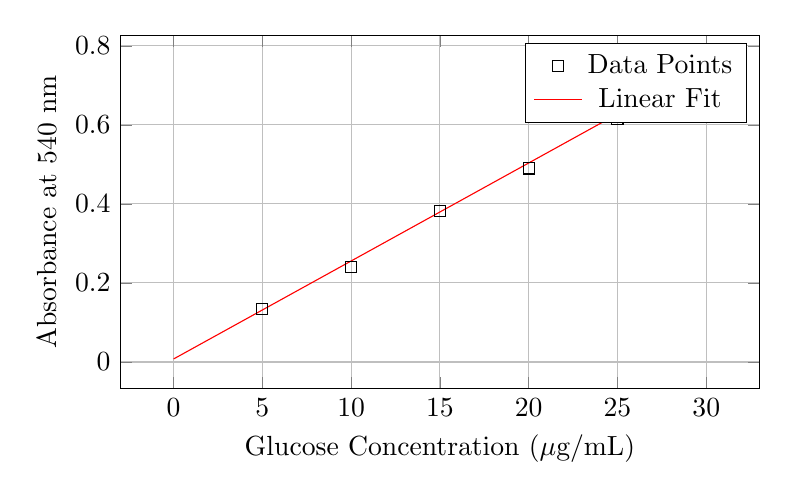
\begin{tikzpicture}
        \begin{axis}[
            xlabel={Glucose Concentration ($\mu$g/mL)},
            ylabel={Absorbance at 540 nm},
            grid=major,
            width=0.8\textwidth,
            height=0.5\textwidth
        ]
        \addplot[
            only marks,
            mark=square,
            ]
            coordinates {
            (5,0.1347)(10,0.2393)(15,0.3820)(20,0.4897)(25,0.6160)
            };
        \addplot[
            color=red,
            domain=0:30,
            samples=100,
            ]
            {0.0248*x + 0.0075};
        \legend{Data Points, Linear Fit}
        \end{axis}
    \end{tikzpicture}
    \caption{Curve of Absorbance vs Glucose Concentration with Linear Fit (m = 0.0248, c = 0.0075)}
\end{figure}
\subsubsection{Calculating Glucose Concentration in Unknown Sample}
From the linear fit equation of the standard curve, we can calculate the glucose concentration in the unknown sample using its absorbance value. \\
For Unknown Sample with average absorbance = $\frac{0.243 + 0.234 + 0.215}{3} = 0.2307$ \\
Using the linear fit equation: \\
$$\text{Absorbance} = m \times \text{Concentration} + c$$
$$0.2307 = 0.0248 \times \text{Concentration} + 0.0075$$
$$\text{Concentration} = \frac{0.2307 - 0.0075}{0.0248} \approx 9.05 \mu g/mL$$
\subsubsection{Conclusion}
The glucose concentration in the unknown sample was estimated using the GOD-POD assay and found to be approximately 9.05 $\mu$g/mL based on the absorbance measurement and the standard curve generated from known glucose concentrations.
\end{document}
